\subsection{Reducción de la dimensionalidad}

Como se ha podido observar, nuestro conjunto de datos no destaca por la existencia de componentes con alta correlación con las variables objetivo, un hecho que dificultará la obtención de resultados destacables. Mediante la reducción de dimensionalidad y el Análisis de Componentes Principales (PCA) se buscará una combinación lineal de las variables originales que capture la mayor cantidad de variabilidad en los datos posible. Esto se logra a través del uso de componentes principales.
\newline

Para no implementar manualmente el Análisis de Componentes Principales se ha optado por usar una funcionalidad de la librería de \cite{Scikit-learn}. Se empezará el estudio con el análisis de los autovalores, también conocidos como eigenvalues. Para realizar el estudio se ha generado la representación gráfica de la cantidad de varianza explicada por cada componente principal. Esta representación, también conocida como Scree Plot se puede visualizar en la Figura \ref{Conjunto-Datos-Scree-Plot}.

\begin{figure}[H]
    \centering
    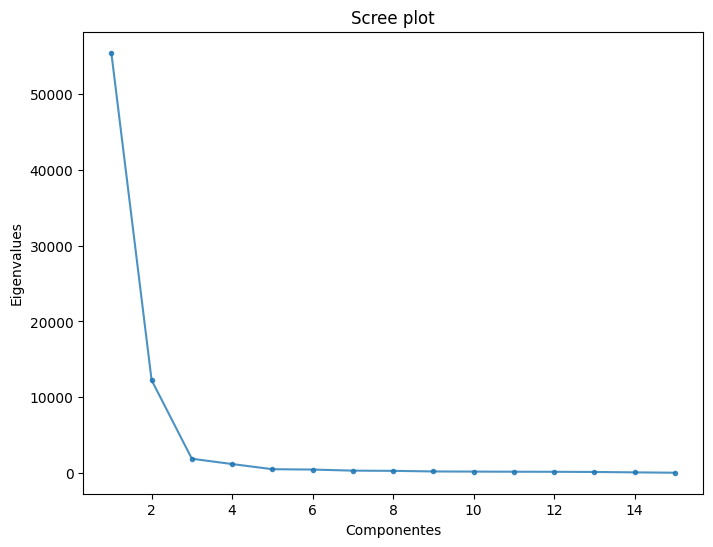
\includegraphics[width=\figsize]{images/screePlot.png}
    \caption{Análisis de Componentes Principales: Scree Plot}
    \label{Conjunto-Datos-Scree-Plot}
\end{figure}

A simple vista se puede evaluar la bondad de ajuste del modelo de PCA. Podemos ver como la mayor parte de la varianza de los datos originales se explica en las primeras componentes, lo que nos permite deducir que el modelo de PCA tiene un buen ajuste. Además, si entramos un poco más en detalle, podemos observar como el número óptimo de componentes principales es 8, ya que en ese punto, encontramos una estabilización de la gráfica, hecho que nos permite afirmar, que usando más de 8 componentes principales estamos perdiendo varianza explicada. Estas conclusiones se han podido comprobar con el gráfico de la Figura \ref{Conjunto-Datos-Varianza-Explicada}. Se puede ver como a partir de la tercera componente, la varianza explicada se mantiene y, por lo tanto, añadir más componentes nos generara ruido en el resultado final.

\begin{figure}[H]
    \centering
    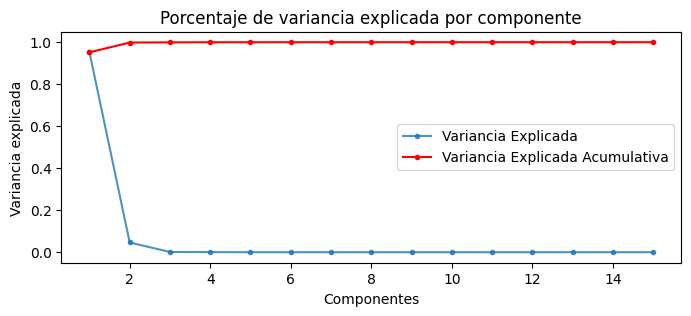
\includegraphics[width=\figsize]{images/varianzaExplicada.png}
    \caption{Análisis de Componentes Principales: Varianza Explicada}
    \label{Conjunto-Datos-Varianza-Explicada}
\end{figure}

El estudio ha finalizado buscando patrones con 2 y 3 componentes. Para realizar el estudio se han generado las Figuras \ref{Conjunto-Datos-Scatter-Plot-2} y \ref{Conjunto-Datos-Scatter-Plot-3}. De ambas visualizaciones podemos sacar las mismas conclusiones, no existen patrones en los datos que nos permitan ajustar fácilmente una recta de regresión, un hecho que va en sintonía con nuestras hipótesis, será altamente complicado obtener resultados satisfactorios debido a la gran variabilidad de los datos.

\begin{figure}[H]
    \centering
    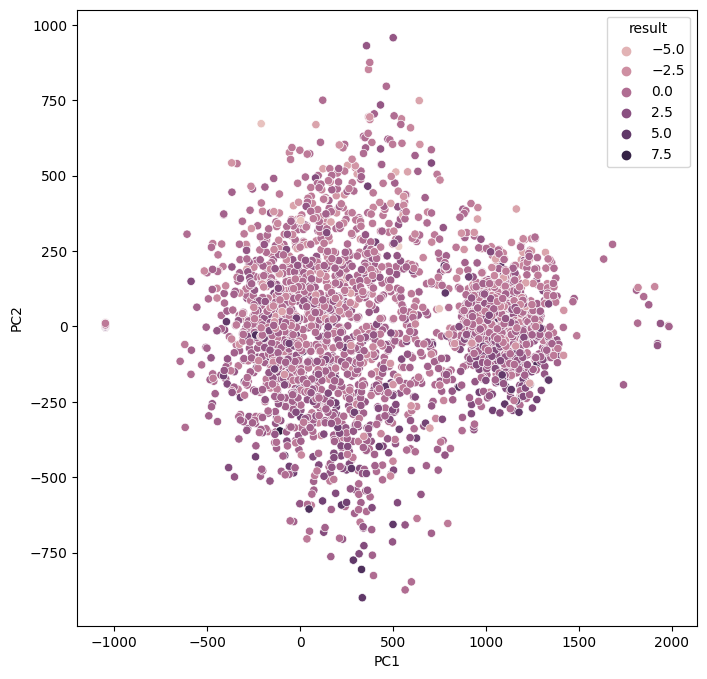
\includegraphics[width=\figsize]{images/scatterPlotPCA2.png}
    \caption{Análisis de Componentes Principales: Dispersión 2 Componentes}
    \label{Conjunto-Datos-Scatter-Plot-2}
\end{figure}

\begin{figure}[H]
    \centering
    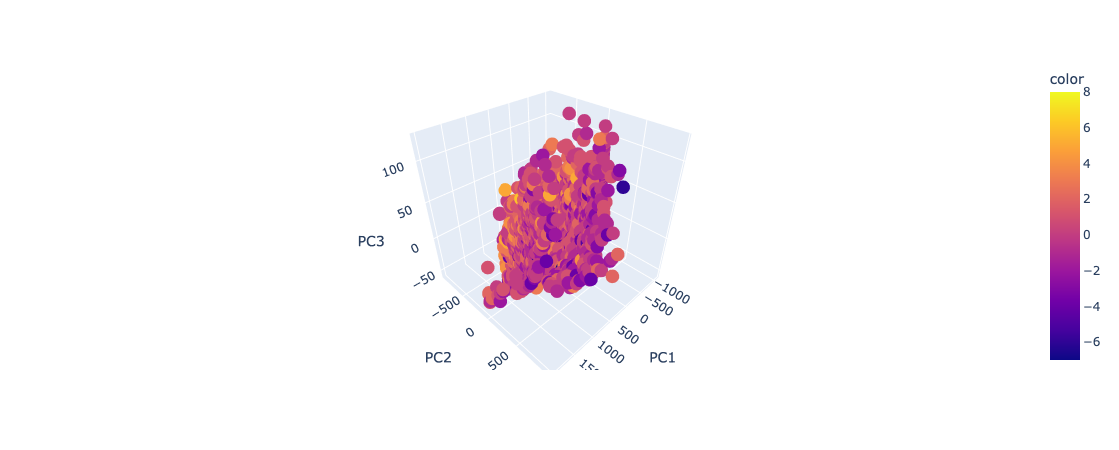
\includegraphics[width=\figsize]{images/scatterPlotPCA3.png}
    \caption{Análisis de Componentes Principales: Dispersión 3 Componentes}
    \label{Conjunto-Datos-Scatter-Plot-3}
\end{figure}